% Created 2017-01-19 Thu 17:34
\documentclass[11pt]{article}
               %\usepackage[scaled=0.88]{beraserif}
               %\usepackage[scaled=0.85]{berasans}
               %\usepackage[scaled=0.84]{beramono}
               \renewcommand{\rmdefault}{pplx} % rm
               \linespread{1.05}        % Palatino needs more leading
               \usepackage[scaled]{helvet} % ss
%               \usepackage{courier} % tt
               \usepackage{eulervm} % a better implementation of the euler package (not in gwTeX)
               \normalfont
               \usepackage[T1]{fontenc}
\usepackage[utf8]{inputenc}
\usepackage[T1]{fontenc}
\usepackage{fixltx2e}
\usepackage{graphicx}
\usepackage{grffile}
\usepackage{longtable}
\usepackage{wrapfig}
\usepackage{rotating}
\usepackage[normalem]{ulem}
\usepackage{amsmath}
\usepackage{textcomp}
\usepackage{amssymb}
\usepackage{capt-of}
\usepackage{hyperref}
\usepackage{minted}
\author{Kangwei Ling 5140219295}
\date{\today}
\title{Project: Smallc Compiler}
\hypersetup{
 pdfauthor={Kangwei Ling 5140219295},
 pdftitle={Project: Smallc Compiler},
 pdfkeywords={},
 pdfsubject={},
 pdfcreator={Emacs 25.1.1 (Org mode 8.3.6)}, 
 pdflang={English}}
\begin{document}

\maketitle
\tableofcontents


\section{Lexical Analysis}
\label{sec:orgheadline5}
In this project, I use \emph{flex} to do lexical analysis, which scans through the
source code text file and generates token stream.
With the language specification, it's very easy to write down the lexical rules
for flex to work on. In addition, the token type can be found in the header file
generated from \emph{yacc / bison}.
\subsection{Keywords}
\label{sec:orgheadline1}
The rules for keywords should be put before identifiers, so that keywords will
not be parsed as identifiers.
\begin{minted}[]{text}
"int"         return(TYPE);
";"         return(SEMI);
","         return(COMMA);
"("         return(LP);
")"         return(RP);
"["         return(LB);
"]"         return(RB);
"{"         return(LC);
"}"         return(RC);
"struct"      return(STRUCT);
"return"      return(RETURN);
"if"          return(IF);
"else"        return(ELSE);
"break"       return(BREAK);
"continue"    return(CONT);
"for"         return(FOR);
\end{minted}
\subsection{Identifiers and Integers}
\label{sec:orgheadline2}
An identifier is a character string consisting of alphabetic characters, digits
and the underscore. Digits can't be the first character. Use the notation of
lex, it can be write down as,
\begin{minted}[]{text}
id    [_a-zA-Z][_a-zA-Z0-9]*
\end{minted}
For numbers, to support 3 format (decimal, octal, hexadecimal), the following
notation is used,
\begin{minted}[]{text}
integer ([0-9]+|0[xX][0-9a-f]+)
\end{minted}
Thus the rules for identifiers and integers can be written as,
\begin{minted}[]{text}
{integer}       { save_num(); return(INT); }
{id}        { save_str(); return(ID);  }
\end{minted}
The two \texttt{save\_} function is defined to save the \texttt{yytext} as token value. As for
integers, a transformation from string to int is done with the limit checked
(-2\(^{\text{31}}\), 2\(^{\text{31}}\)).
\begin{minted}[]{c}
void save_num()
{
    try {
      yylval.ival = stoi(string(yytext), 0, 0); // autodetect base
    } catch (std::invalid_argument& e) {
      std::cerr << "Error token: "<< yytext << " found at line: " << curr_lineno
            << ": invalid number."<< endl;
      yylval.ival = 0;
    } catch (std::out_of_range& e) {
    std::cerr << "Error token: "<< yytext << " found at line: " << curr_lineno
          << ": out of range( -2^(31), 2^(31) )."<< endl;
    yylval.ival = 0;
    }
}
\end{minted}
\subsection{Operators}
\label{sec:orgheadline3}
There are many valid operators for \emph{smallc} language. A careful naming approach
must be adopted. I use a \textbf{L} prefix for logical operators and \textbf{B} prefix for
binary operators. A suffix of \textbf{ASSIGN} is used to denote \emph{op and assign}
operators. Below is a small snippet of this part.
\begin{minted}[]{text}
"."    { save_str(); return(DOT); }
"+"    { save_str(); return(ADD); }
">>"   { save_str(); return(SHR); }
">"    { save_str(); return(GT); }
">="   { save_str(); return(GTE); }
"&"    { save_str(); return(B_AND); }
"&&"   { save_str(); return(L_AND); }
"="    { save_str(); return(ASSIGN); }
"&="   { save_str(); return(AND_ASSIGN); }
">>="   { save_str(); return(SHR_ASSIGN); }
"!"     { save_str(); return(L_NOT); }
"--"    { save_str(); return(P_SUB); }
\end{minted}
It's important to pay attention to binary minus and unary minus, but in lexical
analysis, there is no way to tell whether it's a binary one or unary one.
Therefore, this job is delayed to syntax analysis.
\begin{minted}[]{text}
    /* Minus(-) need to be processed in parser */
"-"     { return(SUB);}
\end{minted}
\subsection{Line Number}
\label{sec:orgheadline4}
Line number is very important for developing and debugging, thus it's necessary
to save the line number when scanning for tokens.
\begin{minted}[]{text}
\n  ++curr_lineno;
\end{minted}
Whenever a newline symbol is detected, the variable \texttt{curr\_lineno} is updated,
this value is also used when creating abstract syntax tree nodes in syntax analysis.
\section{Syntax Analysis}
\label{sec:orgheadline8}
\subsection{Abstract Syntax Tree}
\label{sec:orgheadline6}
I create a abstract syntax node class for every possible
production. All classes inherit from \texttt{AstNode} class,
\begin{minted}[]{cpp}
class AstNode {
protected:
    int line_number;
public:
    AstNode();
    virtual ~AstNode() { }
    virtual void dump(ostream& os, int n) = 0;
    int get_line_number();
};
\end{minted}

Each node must have a line number for debugging, and a \texttt{dump} method to print
out necessary information of this node. I implemented \texttt{dump} method as to print
out the source code that generate this node, to verify the correctness of the
parsing process.Below is a simple inherit class diagram.

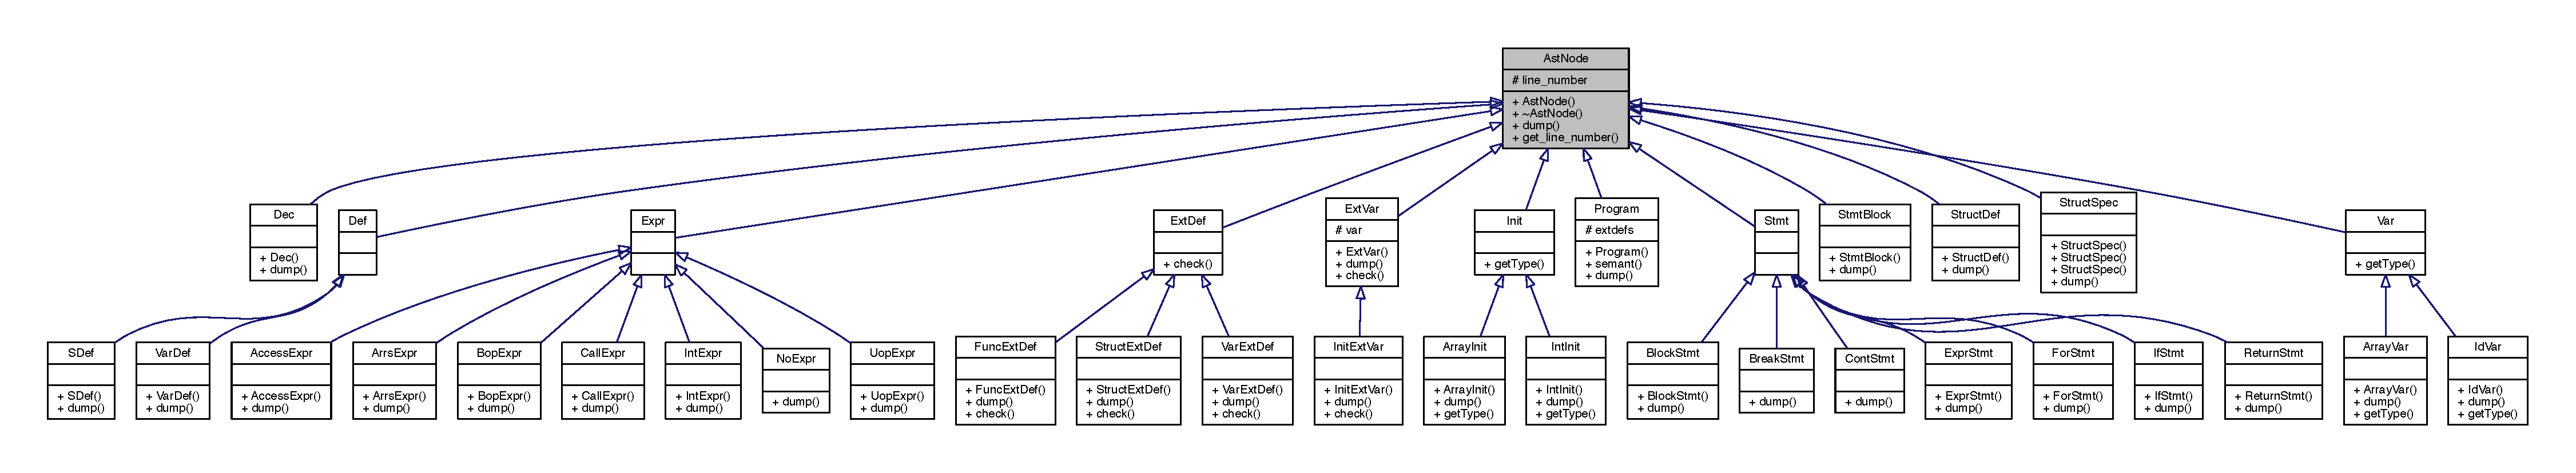
\includegraphics[width=.9\linewidth]{img/class.pdf}

The detail of each class is in the source code.
\subsection{Bison and Grammar}
\label{sec:orgheadline7}
\emph{Bison} is the tool used to generate a parser from given grammars. In this
project, I associate each production with semantic actions so that the abstract
syntax tree is created during the parsing process.

The types of terminals and non-terminals are declared in yylval union.
\begin{minted}[]{c}
%union {
    int ival;
    std::string* sval;
    Program* program;
    ExtDefList* extdefs;
    ExtDef* extdef;
    ExtVar* extvar;
    ExtVarList* extvars;
    SExtVar* sextvar;
    SExtVarList* sextvars;
    StructSpec* stspec;
    Paras* paras;
    StmtBlock* stmtblock;
    StmtList* stmts;
    Stmt* stmt;
    DefList* defs;
    Def* def;
    StructDef* stdef;
    StructDefList* stdefs;
    SDec* sdec;
    SDecList* sdecs;
    Dec* dec;
    DecList* decs;
    Var* var;
    Init* init;
    Arrs* arrs;
    Args* args;
    Expr* exp;
}
\end{minted}

All operator terminals have \texttt{sval} (pointer to string) value to be stored in
\texttt{BopExpr} node class. For non-terminals, they have corresponding class type.

For simplicity, I made a little tweak to \texttt{EXTDEF} production for functions.
\begin{minted}[]{text}
EXTDEF -> TYPE EXTVARS SEMI
        | STSPEC SEXTVARS SEMI
        | TYPE ID LP PARAS RP STBLOCK     (substitute FUNC in)
\end{minted}

For operator precedences, just implement them as the specification says.
\begin{minted}[]{text}
%right ASSIGN ADD_ASSIGN SUB_ASSIGN MUL_ASSIGN DIV_ASSIGN AND_ASSIGN XOR_ASSIGN OR_ASSIGN SHL_ASSIGN SHR_ASSIGN
%left L_OR
%left L_AND
%left B_OR
%left B_XOR
%left B_AND
%left EQ NEQ
%left GT GTE LT LTE
%left SHL SHR
%left ADD SUB
%left MUL DIV MOD
%right UMINUS L_NOT P_ADD P_SUB B_NOT
%left DOT LP RP LB RB

%right THEN ELSE
\end{minted}
\begin{enumerate}
\item binary minus and unary minus

To solve this problem, just set the precedence over the specific production
of UMINUS
\begin{minted}[]{text}
| SUB   EXPS %prec UMINUS    { $$ = new UopExpr(*$1, $2); }
\end{minted}

\item if else

Note that the \texttt{else} should be bond with the last if, using \texttt{\%right THEN
   ELSE} associativity and precedence, the rule below solve this problem.
\begin{minted}[]{text}
| IF LP EXP RP STMT %prec THEN { $$ = new IfStmt($3, $5); }
| IF LP EXP RP STMT ELSE STMT { $$ = new IfStmt($3, $5, $7); }
\end{minted}
\end{enumerate}

\section{Semantic Analysis}
\label{sec:orgheadline18}
\subsection{Symbol Table}
\label{sec:orgheadline9}
Symbol Table is a mapping from symbols to their symbol values. In my
implementation, symbol table is just a wrapper of mapping from string to
template type, meanwhile support scope actions (enter a scope, exit a scope,
lookup a symbol, etc).

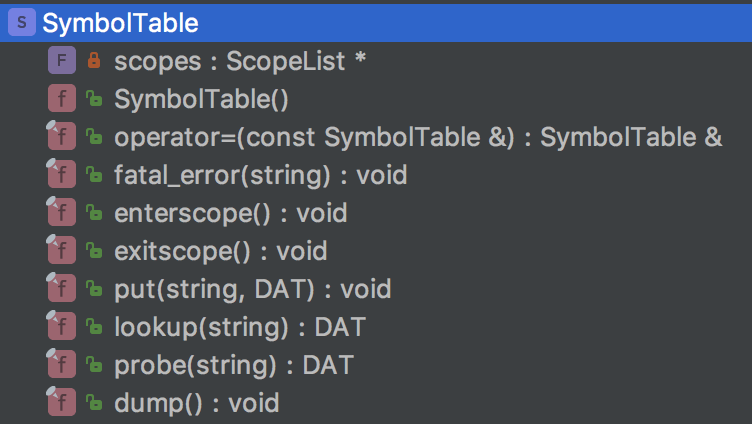
\includegraphics[width=.9\linewidth]{img/symtab.png}

The underlying scope is defined as follows.
\begin{minted}[]{cpp}
using Scope = std::unordered_map<string, DAT>;
using ScopeList = std::list<Scope>;
\end{minted}

\begin{description}
\item[{lookup}] lookup the symbol in the symbol table, if it's not found in the
current scope, search in the previous scope ( next entry of the list). This
method is used when we using an identifier in places other than declarations.
\item[{probe}] only look for the symbol in the current scope. As an identifier can
be redeclared in different scope, so we only search in the current scope
when do declarations.
\end{description}
\subsection{Semantic Check}
\label{sec:orgheadline12}
Four different symbol table is used in my implementation.
\begin{minted}[]{cpp}
SymbolTable<Var*> IntVarTbl;
SymbolTable<StructSpec*> StVarTbl;
SymbolTable<StructSpec*> StSpecTbl;
SymbolTable<FuncExtDef*> funcTbl;
\end{minted}
The \texttt{IntVarTbl} is used for integer and integer array variables, \texttt{StVarTbl}
for struct variables, \texttt{funcTbl} for function identifiers. In addition,
\texttt{StSpecTbl} is a mapping from struct tag to struct specification, for
example,
\begin{minted}[]{c}
struct A {
   int a;
};
\end{minted}
there will be a mapping from *"A"* to this struct specification. Note that, for
struct variables (declared ones), their id is also mapping to the corresponding
spec.

\subsubsection{Helper Functions}
\label{sec:orgheadline10}
I also introduced some help functions to facilitate the semantic analysis
process.

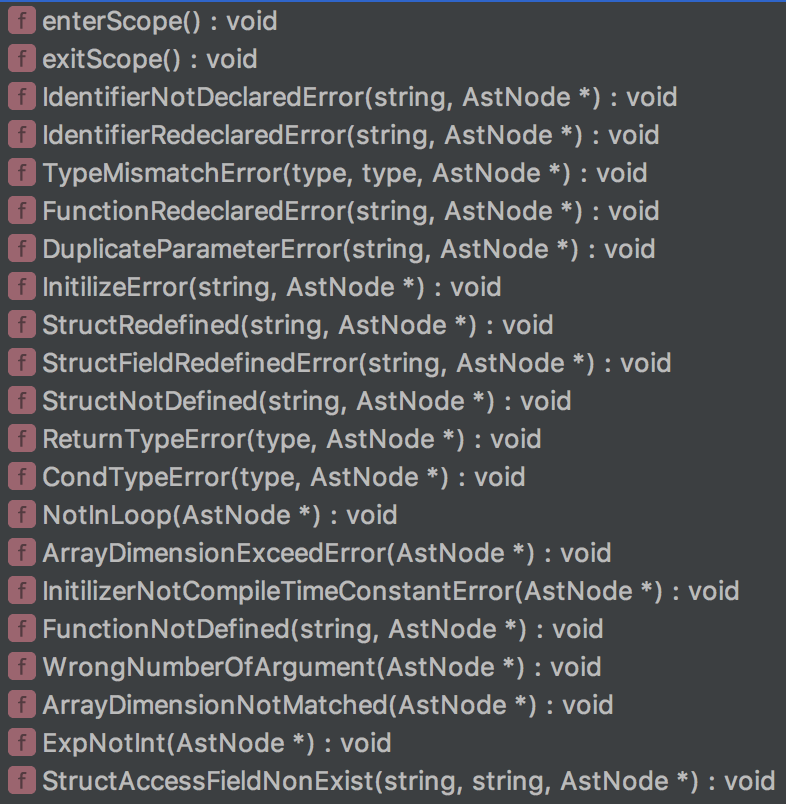
\includegraphics[width=.9\linewidth]{img/error.png}

\texttt{enterscope} and \texttt{exitscope} are just wrapper of symbol table's scope
functions, they are used to control the scope of multiple tables. The others
are just error functions, which normally takes a string and \texttt{AstNode} as
arguments and handle errors. The \texttt{AstNode} is used to get the line number of
the error point. All errors will to put into a \texttt{stringstream} and update
\texttt{semant\_errors}.
\begin{minted}[]{cpp}
static ostringstream err;
static int semant_errors = 0;
\end{minted}
Upon finishing semantic checking, if there are more than one semantic
errors, then the program will no proceed to code generation.

\subsubsection{Checking}
\label{sec:orgheadline11}
Semantic check is started by calling \texttt{semant} method of the \texttt{Program} class,
which is the final ast root. Then it will recursively check all extdefs.

\begin{enumerate}
\item dimension of arrays will be no more than 2.

This can be done by checking the \texttt{ArrayVar}. The \texttt{Var} part of \texttt{ArrayVar}
must have dimension less than 2, with normal scalar having dimension of 0.
\begin{minted}[]{cpp}
if (this->var->getDim() >= 2)
    ArrayDimensionExceedError(this);
\end{minted}

\item initializer compatibility.

A integer variable can not be initialized with an array (such as \{1,1\}),
vice versa. This is done by checking their dimensions.
\begin{minted}[]{cpp}
if (this->var->getType() != this->init->getType() || 
    this->var->getSize() < this->init->getSize()) {
    InitilizeError("Incompatible initializer", this);
 }
\end{minted}

\item variables and functions should be declared before usage.

variables and functions is only used in expressions. When checking, their
identifiers are used to lookup in the symbol table. If not found, an
error occurs.

\item variables and functions should not be re-declared.

just like the previous one, search with their identifier to check if
exists, but only search in current scope (\texttt{probe}). If non exists, we are
all fine. (All symbol table need to be searched).

\item Reserved words.

This is done in lexical part, as reserved words will be firstly parsed as
keyword tokens, not identifiers.

\item Program must contain a function int main() to be the entrance

Just check the \texttt{funcTbl} after checking the extdefs.
\begin{minted}[]{cpp}
FuncExtDef* MainFunc = funcTbl.lookup("main");
if (MainFunc == NULL || MainFunc->getParamCount() != 0) {
    ++semant_errors;
    err << "Program must contain a function int main()!" << endl;
}
\end{minted}

\item The number and type of variable(s) passed should match the definition of
the function.

While checking for \texttt{CallExpr}, check if the number of arguments equals to the
function's parameter counts, and check if all arguments give a int
result.
\begin{minted}[]{cpp}
int n_args_prov = this->args->size();
int n_args_need = func->getParamCount();
if (n_args_need != n_args_prov)
    WrongNumberOfArgument(this);
 // check arguments
for (Expr* exp: *this->args) {
    ExprType::type tp = exp->check();
    if (tp != ExprType::INTEGER)
        ExpNotInt(exp);
}
\end{minted}

\item Use \texttt{[]} operator to a non-array variable is not allowed.

Compare the dimension of variable with the \texttt{Arrs} size (number of
indices).
\begin{minted}[]{cpp}
int dim = v->getDim();
int ac = this->arrs->size();
if (dim != ac) {
    ArrayDimensionNotMatched(this);
\end{minted}

\item The \texttt{.} operator can only be used to a struct variable.

Because I use different symbol table for struct variable and int
variable, this is solved.

\item \texttt{break} and \texttt{continue} can only be used in a for-loop.

I keep a global count for loops. Whenever I entered a for-loop,
increment that count. Whenever done checking a for-loop, decrement it.
If the count is 0 when checking node of \texttt{break} or \texttt{continue}, there
must be an error.

\item Right-value can not be assigned by any value or expression.

When check for Binary OP nodes, if the operator is associated with
assignment, then check if the left expression is an lvalue. Only array
access and struct access are lvalues, so this is not so difficult.

\begin{minted}[]{cpp}
// check if lval
if (this->op.find("=") != std::string::npos && this->op != "=="
        && this->op != ">=" && this->op != "<="
        && this->op != "!=") {
    if (!this->lexp->isLval()) {
        ++semant_errors;
        err << "line " << this->get_line_number() << " " <<  << "error: "
            << "not an lvalue" << endl;
    }
}
\end{minted}

\item The condition of \texttt{if} statement should be an expression with \texttt{int} type.

Every expression has a type, the semantic checking of expression will
return its type.
\begin{minted}[]{cpp}
ExprType::type cond_tp = this->cond->check();
if (cond_tp != ExprType::INTEGER)
    CondTypeError(cond_tp, this);
\end{minted}

\item The condition of \texttt{for} should be an expression with \texttt{int} type or
\(\epsilon\).

The \texttt{BLANK} type is returned by empty expression.
\begin{minted}[]{cpp}
ExprType::type cond_tp = this->cond->check();
if (cond_tp != ExprType::INTEGER && cond_tp != ExprType::BLANK)
    CondTypeError(cond_tp, this);
\end{minted}

\item Only expression with type \texttt{int} can be involved in arithmetic.

This one can be checked inside \texttt{CallExpr} , \texttt{ArrsExpr} and \texttt{AccessExpr}.
As other than those nodes, we only have integers.

\item global initializer should be compile time constant.

The initializer of global variables(int and int arrays) can not contain
\texttt{CallExpr}, \texttt{ArrsExpr} or \texttt{AccessExpr}.

\begin{minted}[]{cpp}
if (!this->init->isConstant())
    InitilizerNotCompileTimeConstantError(this->init);
\end{minted}
\end{enumerate}

\subsection{Annotation}
\label{sec:orgheadline17}
\subsubsection{Indirect information replacement}
\label{sec:orgheadline13}
When doing semantic checking, I also annotate some ast nodes like struct
declarations(with full specification), array access(with var definition),
struct access(with full specification)  and function calls( with function definition) so that in the following phases I don't need
to look up them in symbol table.
\subsubsection{Compile time constant folding}
\label{sec:orgheadline14}
The initializer of global variables(int var, int array) should be able to be
computed at compile time. And the value is used to generate mips code.

I introduced an \texttt{eval} method for expressions, this method will get the
value of a constant expression during semantic analysis.

The \texttt{eval} will only evaluate for binary OP and unary OP and int constant
expression. For \texttt{ArrsExpr}, if it is an scalar var access(there is no
subscript access to array), then return the value of \texttt{var} (which I already
put it here during indirect information replacement), the default value of
\texttt{var} is 0.

The value of an \texttt{Init} (either an int init or array init) will be stored in
a vector (for int init, there is only one element), the value is computed
by a method \texttt{eval},

\begin{minted}[]{cpp}
void IntInit::eval() {
    int v = this->exp->eval();
    //cout << "# compute: " << v << endl;
    value->push_back(v);
}

void ArrayInit::eval() {
    for (Expr* exp: *this->args) {
        int v = exp->eval();
        //cout << "# compute: " << v << endl;
        value->push_back(v);
    }
}
\end{minted}

Note that, after compute compile time constant for global variables, the
value of a global var should be updated with its init value, so that the
future usage of this value during eval is  correct.

\begin{minted}[]{cpp}
this->init->eval();

// code below is associate value with int var. 
// array value value will never been accesses
// during eval expression
IntInit* intinit = dynamic_cast<IntInit*>(this->init);
if (intinit != NULL) {
    (dynamic_cast<IdVar*>(this->var))->value = (*(intinit->value))[0];
    return;
}
\end{minted}
\subsubsection{Struct Specification flatten}
\label{sec:orgheadline15}
Because in the grammar, specification for struct is wrapped in two layers,
it will be very useful for calculating offset if the fields are in a flatten
list.

\begin{minted}[]{text}
for (StructDef* structdef : *this->sdefs) {
    structdef->check();
    fields.insert(fields.end(), 
           structdef->sdecs->begin(), structdef->sdecs->end());
}
\end{minted}
\subsubsection{read and write}
\label{sec:orgheadline16}
These two function is added into \texttt{funcTbl} at the beginning.

\begin{minted}[]{cpp}
Paras* pp = new Paras;
pp->push_front("x");
FuncExtDef* read = new FuncExtDef("read", pp, nullptr);
FuncExtDef* write = new FuncExtDef("write", pp, nullptr);
funcTbl.put("read", read);
funcTbl.put("write", write);
\end{minted}

When checking for function call, \texttt{read} call must be called with lvalue
argument!

\begin{minted}[]{cpp}
if (this->id == "read" && !exp->isLval()) {
    ++semant_errors;
    err << "line " << exp->get_line_number() << " " << "error: "
    << "not an lvalue" << endl;
}
\end{minted}
\section{IR Generation}
\label{sec:orgheadline27}
For this project, I use three address code as intermediate representation,
this form of IR is very close to the assembly language so that it will be very
easy to transform into final assembly code.

Every TAC class inherit from \texttt{Instruction} class.
\begin{minted}[]{cpp}
class Instruction {
protected:
    char printed[128];
public:
    virtual ~Instruction() {}
    virtual void Print();
    virtual void EmitSpecific(Mips *mips) = 0;
    virtual void Emit(Mips *mips);
};
\end{minted}
The printed array is the string representation of the instruction(for printing
three address code out).

Below is a small IR snippet:

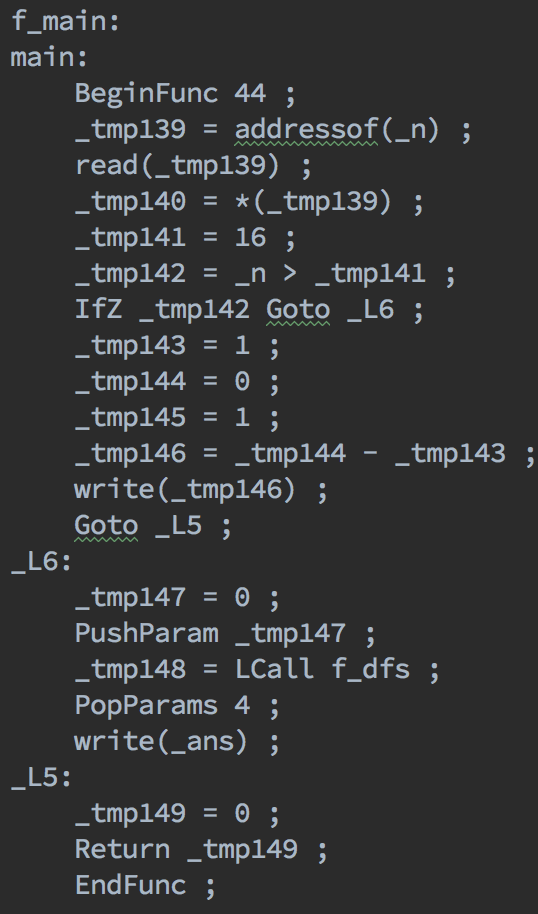
\includegraphics[width=.9\linewidth]{img/ir.png}

\subsection{Three Address Code}
\label{sec:orgheadline19}
The following three address code classes are used in this project.
\begin{minted}[]{cpp}
class LoadConstant; // load immediate
class Assign;
class Load;
class Store;
class BinaryOp;
class Label;
class Goto;
class IfZ;
class BeginFunc;
class EndFunc;
class Return;
class PushParam;
class RemoveParams;
class LCall;
class GlobalData;
class ReadInt;
class WriteInt;
class LoadAddress;
\end{minted}
It's very clear what does each one means, you can tell by its name. The
detail of each class is in file \texttt{tac.h/.cpp}.

\subsection{Location}
\label{sec:orgheadline20}
A Location object is used to identify the operands to the various TAC
instructions. A Location is either \texttt{fp} or \texttt{gp} 
relative (depending on whether in stack or global segment) 
and has an offset relative to the base of that segment.
For example, a declaration for integer num as the first local
variable in a function would be assigned a Location object
with name "num", segment fpRelative, and offset -8.
\begin{minted}[]{cpp}
typedef enum {fpRelative, gpRelative} Segment;

class Location
{
protected:
    const string variableName;
    Segment segment;
    int offset;

public:
    Location(Segment seg, int offset, const string name);

    const string GetName() const     { return variableName; }
    Segment GetSegment() const      { return segment; }
    int GetOffset() const           { return offset; }

    bool locationRef;

    bool operator==(const Location& that) const {
        return this->GetName() == that.GetName() &&
       this->GetSegment() == that.GetSegment() &&
       this->GetOffset() == that.GetOffset();
    }
};
\end{minted}
Each TAC class is associated with one or more \texttt{Location} (i.e. src and dst)
\subsection{IR generator}
\label{sec:orgheadline21}
  The CodeGenerator class is used to build TAC
instructions (using the Tac class and its subclasses) and store the
instructions in a sequential list when traversing the abstract syntax tree for
IR generation, ready for further processing or translation to MIPS as part of
final code generation. 

This class has two code lists, one for global data, another for code segment.
\begin{minted}[]{cpp}
std::list<Instruction*> *code;
std::list<Instruction*> *data;
\end{minted}
Also, this class holds a symbol table mapping from variable name to their
locations (including temp vars). Besides, it provides utility functions to
use the stack and global area, as well as generate label and temp vars.
\begin{minted}[]{cpp}
string NewLabel();
Location *GenGlobalVar(const string name, unsigned int size, vector<int> *init);
Location *GetNewLocationOnStack(const string name);
Location *GetNewBulkLocationOnStack(const string name, unsigned int size);
Location *GenTempVar();
\end{minted}
Apart from all these, other methods are used to generate corresponding TAC
instruction. The details of the implementation is in file \texttt{IRgen.h/cpp}.
\subsection{emit}
\label{sec:orgheadline26}
The TAC instruction list is built up upon traversing the abstract syntax
tree. The \texttt{emit} method of ast classes does this job. The implementation can
be found in file \texttt{ast\_emit.h}.
\subsubsection{Global Variables}
\label{sec:orgheadline22}
Upon start, it'will firstly generate tac for global variables(int, int array,
struct). Actually these three are basically the same because they only use a
sequence of 4-bytes memory. With enough information provided in the ast node,
use \texttt{IRGenerator}'s \texttt{GenGlobalVar} method is very straightforward.
\subsubsection{Function}
\label{sec:orgheadline23}
For function defs, firstly a label tac will be generated for that function,
locations of its parameters will be set, then its body will be emit.
\begin{minted}[]{cpp}
void FuncExtDef::emit(IRGenerator *irg)
{
    irg->NewScope();

    string tmp = "f_" + this->id;
    irg->GenLabel(tmp);

    if (this->id == "main")
        irg->GenLabel("main");

    BeginFunc* bf = irg->GenBeginFunc();

    // gen stack space for parameter
    int onStackParam = 0;
    for (const string &p : *params) {
        irg->InsertLocation(p, new Location(fpRelative, 4 + onStackParam * 4, p));
        ++onStackParam;
    }

    this->stmtBlock->emit(irg);

    bf->SetFrameSize(irg->currentStackSize * 4);
    irg->GenEndFunc();

    irg->RemoveScope();
}
\end{minted}

\subsubsection{Statement}
\label{sec:orgheadline24}
For statement, just follow the definition of the statement and generate
correct tac. For loops to work with \texttt{break} and \texttt{continue}, I kept two
global lists of exit labels and for-loop's update label. Thus \texttt{break} and
\texttt{continue} will be jump to the correct label.
\subsubsection{Expression}
\label{sec:orgheadline25}
The \texttt{emit} method for expressions are a little bit difficult, because I was
torn between reference(addresses) and values.

\begin{enumerate}
\item Binary Operators

For normal binary operators(corresponding mips op exists), just generate
BinaryOp TAC. For logical and "\&\&" and logical or "||", I expand them
into normal operations.
\begin{minted}[]{cpp}
// for logical and &&
 Location* zero = irg->GenLoadConstant(0);

 Location* llres = irg->GenBinaryOp("!=", zero, lres);
 Location* rrres = irg->GenBinaryOp("!=", zero, rres);
 return irg->GenBinaryOp("&", llres, rrres);
\end{minted}
 For operator associated with assignment, firstly the result is
calculated as normal operations, and then an reference location(the
address) is generated via \texttt{emitMemoryLocation}, then a store tac is
generated.

\item Unary Operators

transformed into binary operators. Bitwise negation is transformed into
an XOR with -1.

\item Call function

The arguments will be emit first and PushParam is genrated.(The last
argument is pushed firstly).

\item ArrsExpr (array access)

The \texttt{emitMemoryLocation} method will generate a \texttt{LoadAddress} TAC and the
location contains that address will returned. For normal \texttt{emit} method, a
\texttt{Load} TAC is generated from the memory location. Because arrays are not
allowed to have dimension more than 2, therefore calculation of the
offset is hardcoded
\begin{minted}[]{cpp}
Location* ArrsExpr::emitMemoryLocation(IRGenerator *irg)
{
    Location* base = irg->GetLocation(var->getId());
    Location* baseLoc = irg->GenLoadAddress(base);
    int dim = var->getDim();
    if (dim == 0) {
        baseLoc->locationRef = true;
        return baseLoc;
    } else {
        Location* fourL = irg->GenLoadConstant(4);
        Location* arg0 = arrs->front()->emit(irg);
        Location* baseLoc = irg->GenLoadAddress(base);

        if (dim == 1) {
            Location* fl = irg->GenBinaryOp("+", baseLoc, 
                                    irg->GenBinaryOp("*", arg0, fourL));
            fl->locationRef = true;
            return fl;
        } else {
            // two dimension
            int numInRow = var->getSize();
            Location* col = irg->GenLoadConstant(numInRow);
            Location* arg1 = arrs->back()->emit(irg);
            Location* tmp = irg->GenBinaryOp("+", 
                                irg->GenBinaryOp("*", arg0, col), arg1);

            Location* fl = irg->GenBinaryOp("+", baseLoc, 
                                 irg->GenBinaryOp("*", tmp, fourL));
            fl->locationRef = true;
            return fl;
        }
    }
}
\end{minted}

\item AccessExpr struct field access

This part is very similar to array access (one dimension array);

\item IntExpr

A \texttt{LoadConstant} TAC is genrated with the int value associated with the node.
\end{enumerate}



\section{Code Generation}
\label{sec:orgheadline30}
Once the IR is generated, each TAC will be translated into mips code. If
\texttt{-tac} is in the end of command line arguments, then the TAC codes will be
written to the file, otherwise mips code will be generated.

The code generation work is done with the \texttt{Mips} class.
The Mips class defines an object capable of emitting MIPS
instructions and managing the allocation and use of registers.
It is used by the Tac instruction classes to convert each
instruction to the appropriate MIPS equivalent.

Below is a small generated mips snippet

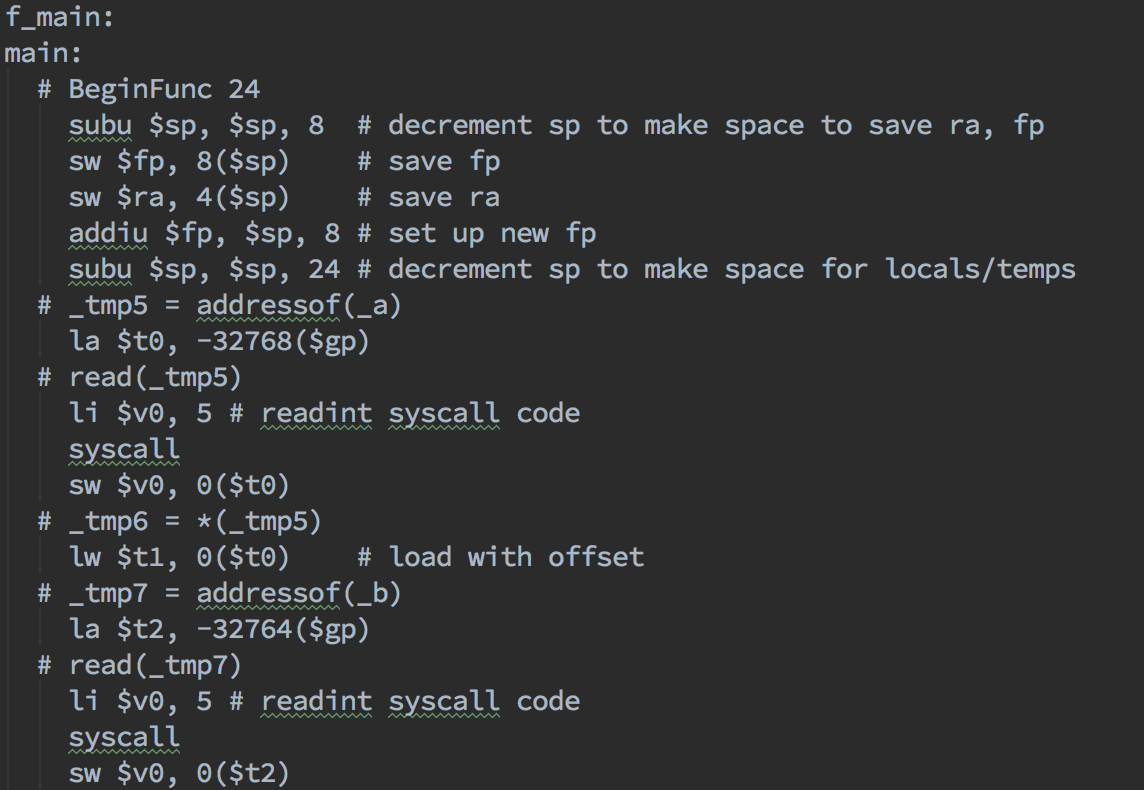
\includegraphics[width=.9\linewidth]{img/mips.png}

\subsection{Instruction Selection}
\label{sec:orgheadline28}
\begin{enumerate}
\item Binary Operation

 For operator: "*", "/", "\%", "+", "-", \label{orgtarget1}", ">", ">=", "<", "<=",
"\texttt{=", "!}", "\&", "\^{}", "|", corresponding mips instructions exist, a mapping
 works well.

\item Load \& Store

\texttt{li} instruction is used for \texttt{LoadConstant}, \texttt{la} is used for
\texttt{LoadAddress}, \texttt{lw} is used for \texttt{Load}, \texttt{sw} is used for \texttt{Store}

\item Others
\texttt{move} instruction for \texttt{Assign}, \texttt{b} for \texttt{Goto}, \texttt{beqz} for \texttt{IfZ}. Details
of functions call are listed in the file \texttt{mips.h/cpp}

\item Read \& Write

syscall of mips is used.
\begin{minted}[]{cpp}
void Mips::EmitRead(Location *dst) {
    Emit("li $v0, 5 # readint syscall code");
    Emit("syscall");
    Register rd = GetRegister(dst);
    Emit("sw $v0, %d(%s)", 0,regs[rd].name);
}

void Mips::EmitWrite(Location *src) {
    Emit("li $v0, 1 # readint syscall code");
    Register r = GetRegister(src);
    Emit("move $a0, %s", regs[r].name);
    Emit("syscall");
}
\end{minted}
\end{enumerate}

\subsection{Register allocation}
\label{sec:orgheadline29}
I used a very basic register policy in this project. A method \texttt{GetRegister}
is used to get a register for use.

  Given a location for a current var, a reason (ForRead or ForWrite)
  and up to two registers to avoid, this method will assign
to a var to register trying these alternatives in order:
\begin{enumerate}
\item if that var is already in a register ("same" is determined
by matching name and same scope), we use that one
\item find an empty register to use for the var
\item find an in-use register that is not dirty.  We don't need
to write value back to memory since it's clean, so we just
 replace with the new var
\item spill an in-use, dirty register, by writing its contents to
    memory and then replace with the new var
For steps 3 \& 4, we respect the registers given to avoid (ie the
other operands in this operation). The register descriptors are
updated to show the new state of the world. If for read, we
load the current value from memory into the register. If for
write, we mark the register as dirty (since it is getting a
new value).
\end{enumerate}
\end{document}